%----------------------------------------------------------------------------------------
%   PACKAGES AND DOCUMENT CONFIGURATIONS
%----------------------------------------------------------------------------------------

\documentclass[a4paper]{book}

\usepackage{siunitx} % Provides the \SI{}{} and \si{} command for typesetting SI units
\usepackage{graphicx} % Required for the inclusion of images
\usepackage{natbib} % Required to change bibliography style to APA
\usepackage{amsmath} % Required for some math elements 
\usepackage{amsfonts}
\usepackage{bbm}
\usepackage{enumerate}
\usepackage{algorithm}
% \usepackage{algorithmic}
\usepackage{algpseudocode}
\setlength\parindent{0pt} % Removes all indentation from paragraphs

% \renewcommand{\labelenumi}{\alph{enumi}.} % Make numbering in the enumerate environment by letter rather than number (e.g. section 6)
\usepackage{geometry}
\geometry{a4paper,scale=0.8}
\usepackage{indentfirst}
\setlength{\parindent}{2em}
\usepackage{times} % Uncomment to use the Times New Roman font
% \usepackage{ctex}
% \usepackage{hyperref}
\usepackage[inline]{enumitem}
\usepackage{listings}
\usepackage[bookmarks]{hyperref}
% \usepackage{mathptmx}
\usepackage[OT1]{fontenc}  % https://tex.stackexchange.com/questions/358261/latex-font-warning-after-updating-to-texlive-2016
% \renewcommand\thechapter{\arabic{chapter}}
% \renewcommand\thesection{\arabic{section}}
% \renewcommand\thesubsection{(\arabic{subsection})}

%----------------------------------------------------------------------------------------
%   DOCUMENT INFORMATION
%----------------------------------------------------------------------------------------

\title{Notes for Reinforcement Learning} % Title

\author{Mhttx} % Author name

\date{\today} % Date for the report

\begin{document} 
\maketitle % Insert the title, author and date
% \pdfbookmark[0]{\contentsname}{toc}%
\tableofcontents
%# -*- coding: utf-8-unix -*-
% !TEX program = xelatex
% !TEX root = ../main.tex
% !TEX encoding = UTF-8 Unicode
\chapter{Introduction}
\label{chap:ch_1_intro}

\section{Reinforcement Learning}
\section{Elements of RL}

\part{Tabular Solution Methods}
%# -*- coding: utf-8-unix -*-
% !TEX program = xelatex
% !TEX root = ../main.tex
% !TEX encoding = UTF-8 Unicode
\chapter{Multi-armed Bandits}
\label{chap:ch_2_Multi-armed_Bandits}

% \section{Multi-armed Bandit Problem}
\section{A k-armed Bandit Problem}
We denote the action selected on time step $t$ as $A_t$, and the corresponding reward as $R_t$. The value then of an arbitrary action $a$, denoted $q_*(a)$, is the expected reward given that $a$ is selected:
\begin{equation}
        q_*(a) \dot{=} \mathbb{E}[R_t|A_t=a]
\end{equation}
We denote the estimated value of action a at time step $t$ as $Q_t(a)$. We would like $Q_t(a)$ to be close to $q_*(a)$.
\section{Action-value Methods}
\textbf{sample-average} method: estimates $q_*(a)$ by averaging the rewards actually received:
\begin{equation}
    Q_t(a) \dot{=} \frac{\sum_{i=1}^{t-1}R_i \cdot \mathbbm{1}_{A_i=a}}{\sum_{i=1}^{t-1}\mathbbm{1}_{A_i=a}}
\end{equation}
As the denominator goes to infinity, by the law of large numbers, $Q_t(a)$ converges to $q_*(a)$.

\textbf{greedy action selection:} 
\begin{equation}
    A_t \dot{=} arg\max_{a}Q_t(a)
\end{equation}

\textbf{$\epsilon$-greedy action selection:}
\begin{equation}
    A_t \dot{=} \begin{cases}
        arg \max_a{Q_t(a)}, \quad with \quad probability \quad 1-\epsilon \\
        a \quad random \quad action, \quad with \quad probability \quad \epsilon 

\end{cases}
\end{equation}
In the limit as the number of steps increases, every action will be sampled an infinite number of times, thus ensuring that all the $Q_t(a)$ converge to $q_*(a)$.

\section{The 10-armed Testbed}

\section{Incremental Implementation}
\begin{equation}
    Q_n \dot{=} \frac{R_1+R_2+\dots+R_{n-1}}{n-1}
\end{equation}

\begin{equation}
\label{eq:update_rule_aveage}
\begin{split}
    Q_{n+1} = & \frac{1}{n}\sum_{i=1}^{n}R_i \\
    =&\frac{1}{n}(R_n+\sum_{i=1}^{n-1}R_i)\\
    =&\frac{1}{n}(R_n+(n-1)\frac{1}{n-1}\sum_{i=1}^{n-1}R_i)\\
    =&\frac{1}{n}(R_n+(n-1)Q_n)\\
    =&Q_n + \frac{1}{n}(R_n-Q_n)
\end{split}
\end{equation}
The general form of \ref{eq:update_rule_aveage} is:
\begin{equation}
    NewEstimate = OldEstimate + StepSize * [Target - OldEstimate]
\end{equation}
Note that the step-size parameter (StepSize, denote as $\alpha$ or $\alpha_t(a)$) used in the incremental method described above changes from time step to time step, here $\alpha_t(a)=\frac{1}{n}$.

\section{Tracking a Nonstationary Problem}
The averaging methods discussed so far are appropriate for \textbf{stationary bandit problems}, that is, for
bandit problems in which the reward probabilities do not change over time. \textbf{In effectively nonstationary cases it makes sense to give more weight to recent rewards than to long-past rewards.} One of the most popular ways
of doing this is to use a \textbf{constant step-size parameter}:
\begin{equation}
    Q_{n+1} \dot{=} Q_n+\alpha[R_n-Q_n]
\end{equation}
This results in $Q_{n+1}$ being a weighted average of past rewards and the initial estimate $Q_1$:
\begin{equation}
\begin{split}
    Q_{n+1} = & Q_{n} + \alpha[R_n-Q_n]\\
            = & \alpha R_n + (1-\alpha)Q_n\\
            = & \alpha R_n + (1-\alpha)[\alpha R_{n-1}+(1-\alpha) Q_{n-1}]\\
            = & \alpha R_n + (1-\alpha)\alpha R_{n-1} +(1-\alpha)^2 Q_{n-1}\\
            = & \alpha R_n + (1-\alpha)\alpha R_{n-1} + (1-\alpha)^2 \alpha R_{n-2} + \\
                            & \cdots+(1-\alpha)^{n-1}\alpha R_1 + (1-\alpha)^n Q_1\\
            = & (1-\alpha)^nQ_1+\sum_{i=1}^{n}\alpha(1-\alpha)^{n-i}R_i
\end{split}
\end{equation}
Note that the weight, $\alpha(1-\alpha)^{n-i}$, given to the reward $R_i$ depends on how many rewards ago, Accordingly, this is sometimes called an \textbf{exponential recency-weighted average}.
eros
Let $\alpha_n(a)$ denote the step-size parameter used to process the reward received after the $n_th$ selection of action $a$. Conditions required to assure convergence with probability 1:
\begin{equation}
\sum_{n=1}^{\infty} \alpha_n(a) = \infty  \quad and \quad \sum_{n=1}^{\infty} \alpha_n^2 \ < \infty
\end{equation}

The first condition is required to guarantee that the steps are large enough to eventually overcome any initial conditions or random fluctuations. The second condition guarantees that eventually the steps become small enough to assure convergence.

Note that both convergence conditions are met for the sample-average case, $\alpha_n(a)=\frac{1}{n}$, but not for
the case of constant step-size parameter, $\alpha_n(a)=\alpha$. In the latter case, the second condition is not met, indicating that \textbf{the estimates never completely converge but continue to vary in response to the most recently received rewards. As we mentioned above, this is actually desirable in a nonstationary environment.}

\section{Optimistic Initial Values}
All the methods we have discussed so far are dependent to some extent on the initial action-value
estimates, $Q_1(a)$. These methods are biased by their initial estimates. The downside is that the initial estimates become, in effect, a set of parameters that must be picked by the user, if only to set them all to zero. The upside is that they provide an easy way to \textbf{supply some prior knowledge}
about what level of rewards can be expected.

Initial action values can also be used as a simple way to encourage exploration. We call this technique for encouraging exploration \textbf{optimistic initial values}. It is not well suited to nonstationary problems because its drive for exploration is inherently temporary. If the task changes, creating a renewed need for exploration, this method cannot help. Indeed, any method that focuses on the initial conditions in any special way is unlikely to help with the general nonstationary case. The beginning of time occurs only once, and thus we should not focus on it too much.

\section{Upper-Confidence-Bound Action Selection}
It would be better to select among the non-greedy actions according to their \textbf{potential for actually being optimal},
taking into account both \textbf{how close their estimates are to being maximal and the uncertainties in those
estimates}. 

\begin{equation}
    A_t \dot{=} arg \max_{a}[Q_t(a)+c\sqrt{\frac{\ln t}{N_t(a)}}]
\end{equation}

The idea of this \textbf{upper confidence bound (UCB)} action selection is that the square-root term is a
measure of \textbf{the uncertainty or variance in the estimate of $a$ ’s value.} The quantity being max’ed over is
thus a sort of upper bound on the possible true value of action $a$, with $c$ determining the confidence level.

One difficulty is in dealing with nonstationary problems. Another difficulty is dealing with large state spaces, particularly when using function approximation.

\section{Gradient Bandit Algorithms}
$H_t(a)$ as a numerical preference of each action $a$. 
\begin{equation}
    \pi_t(a) \dot{=} softmax(H_t(a))\dot{=}\frac{e^{H_t(a)}}{\sum_{b=1}^{k}e^{H_t(b)}}
\end{equation}

\textbf{The Bandit Gradient Algorithm as Stochastic Gradient Ascent:} In exact gradient ascent, each preference $H_t(a)$ would be incremented proportional to the increment’s effect on performance:
\begin{equation}
\label{eq:bga}
    H_{t+1}(a) \dot{=} H_t(a) + \alpha \frac{\partial\mathbb{E}[R_t]}{\partial H_t(a)}
\end{equation}

\begin{equation}
    \mathbb{E}[R_t] = \sum_{b}\pi_t(b)q_{*}(b)
\end{equation}

\begin{equation}
\begin{split}
    \frac{\partial \mathbb{E}[R_t]}{\partial H_t(a)} = & \frac{\partial}{\partial H_t(a)}[\sum_{b}\pi_t(b)q_*(b)]\\
    = & \sum_{b}q_*(b) \frac{\partial \pi_t(b)}{\partial H_t(a)}\\
    = & \sum_{b}(q_*(b)-X_t)\frac{\partial \pi_t(b)}{\partial H_t(a)}
\end{split}
\end{equation}
where $X_t$ can be any scalar that does not depend on $b$, we can include it here because the gradient sums to zero over all the actions, $\sum_b\frac{\partial \pi_t(b)}{\partial H_t(a)}=0$.
\begin{equation}
\begin{split}
    \frac{\partial \mathbb{E}[R_t]}{\partial H_t(a)} = & \sum_b \pi_t(b) (q_*(b)-X_t)\frac{\partial \pi_t(b)}{\partial H_t(a)}/\pi_t(b)\\
    = & \mathbb{E}[(q_*(A_t)-X_t)\frac{\partial \pi_t(A_t)}{\partial H_t(a)}/\pi_t(A_t)] \\
    = & \mathbb{E}[(R_t-\bar{R}_t)\frac{\partial \pi_t(A_t)}{\partial H_t(a)}/\pi_t(A_t)]
\end{split}
\end{equation}
we have $\frac{\partial \pi_t(b)}{\partial H_t(a)}=\pi_t(b)(\mathbbm{1}_{a=b}-\pi_t(a))$, and substituted it.
\begin{equation}
    \frac{\partial \mathbb{E}[R_t]}{\partial H_t(a)}=\mathbb{E}[(R_t-\bar{R}_t)(\mathbbm{1}_{a=A_t}-\pi_t(a))]
\end{equation}
Substituting a sample of the expectation above for the performance gradient in \ref{eq:bga}:
\begin{equation}
    H_{t+1}(a) = H_t(a) + \alpha (R_t-\bar{R}_t)(\mathbbm{1}_{a=A_t}-\pi_t(a))
\end{equation}
%# -*- coding: utf-8-unix -*-
% !TEX program = xelatex
% !TEX root = ../main.tex
% !TEX encoding = UTF-8 Unicode
\chapter{Finit Markov Decision Process}
\label{chap:ch_3_Finit_Markov_Decision_Process}

\section{The Agent-Environment Interface}
\begin{enumerate}
    \item \textbf{finite MDP:} the sets of states, actions and rewards($\mathcal{S, A, R}$) all have a finite number of elements.

    \item \textbf{Markov property:} In this case, the random variables $R_t$ and $S_t$ have well defined discrete probability distributions dependent only on the preceding state and action.
    \begin{equation}
        p(s', r|s, a) \dot{=} Pr\{S_t=s', R_t=r|S_{t-1}=s, A_{t-1}=a\}
    \end{equation}

    \item \textbf{state-transitation probabilities:}
    \begin{equation}
        p(s'|s,a) \dot{=} Pr\{S_t=s'|S_{t-1}=s, A_{t-1}=a\} = \sum_{r \in \mathcal{R}}p(s',r|s,a)
    \end{equation}

    \item \textbf{expected rewards for state–action pairs:}
    \begin{equation}
        r(s,a) \dot{=} \mathbb{E}[R_t|S_{t-1}=s, A_{t-1}=a] = \sum_{r \in \mathcal{R}}r\sum_{s' \in \mathcal{S}}p(s',r|s, a)
    \end{equation}

    \item \textbf{expected rewards for state-action-next-state triplets:}
    \begin{equation}
        r(s,a,s') \dot{=} \mathbb{E}[R_t|S_{t-1}=s,A_{t-1}=a, S_t=s']=\sum_{r \in \mathcal{R}}r\frac{p(s',r, s, a)}{p(s'|s,a)}
    \end{equation}
\end{enumerate}

\section{Goals and Rewards}
\textbf{Reward hypothesis}:That all of what we mean by goals and purposes can be well thought of as the maximization of the expected value of the \textbf{cumulative sum of a received scalar signal} (called reward).

\section{Returns and Episodes}
\begin{enumerate}
    \item \textbf{episodic(episode) tasks:} when the agent–environment interaction breaks naturally into subsequences, which we call episodes. Tasks with episodes of this kind are called episodic tasks.

    \item \textbf{continuing tasks:} the agent–environment interaction does not break naturally into identifiable episodes, but goes on continually without limit.

    \item \textbf{return(simple):}
        \begin{equation}
            G_t \dot{=} R_{t+1}+R_{t+2}+R_{t+3}+\dots+R_T
        \end{equation}

    \item \textbf{discounted return:}
        \begin{equation}
            G_t \dot{=} R_{t+1}+ \gamma R_{t+2} + \gamma^2 R_{t+3} + \dots = \sum_{k=0}^{\infty}\gamma^kR_{t+k+1}
        \end{equation}
    where $\gamma$ is a parameter, $0 \leq \gamma \leq 1$, called the \textbf{discount rate}. As $\gamma$ approaches 1, the return objective takes future rewards into account more strongly; the agent becomes more farsighted.

    \item \textbf{Returns at successive time steps:}
        \begin{equation}
        \begin{split}
            G_t \dot{=} & R_{t+1}+\gamma R_{t+2}+\gamma^2 R_{t+3} + \gamma^3 R_{t+4}+\dots\\
                = &R_{t+1} + \gamma (R_{t+2}+\gamma^1 R_{t+3} + \gamma^2 R_{t+4}+\dots)\\
                = &R_{t+1} + \gamma G_{t+1}
        \end{split}
        \end{equation}

\end{enumerate}

\section{Unified Notation for Episodic and Continuing Tasks}

\section{Policies and Value Functions}
\begin{enumerate}
    \item \textbf{policy:} a mapping from states to probabilities of selecting each possible action. If the agent is following policy $\pi$ at time $t$ , then $\pi(a|s)$ is the probability that $A_t = a$ if $S_t = s$.

    \item \textbf{state-value function for policy $\pi$:} the expected return when starting in $s$ and following $\pi$ thereafter:
        \begin{equation}
            v_{\pi}(s) \dot{=} \mathbb{E}_{\pi}[G_t|S_t=s] \quad \forall s \in \mathcal{S}
        \end{equation}

    \item \textbf{action-value function for policy $\pi$:} the expected return starting from $s$ , taking the action $a$ , and thereafter following policy $\pi$:
        \begin{equation}
            q_{\pi}(s,a) \dot{=} \mathbb{E}_{\pi}[G_t|S_t=s, A_t=a]
        \end{equation}

    \item \textbf{$v_{\pi}(s)$ vs $q_{\pi}(s,a)$:}
        \begin{equation}
            v_{\pi}(s) = \sum_{a \in \mathcal{A}}\pi(a|s)q_{\pi}(s,a)
        \end{equation}

    \item \textbf{Bellman equation for $v_{\pi}$:} It states that the value of the start state must equal the (discounted) value of the expected next state, plus the reward expected along the way. as show in Figure-\ref{fig:dackup_diagram_for_vpi}
        \begin{equation}
        \begin{split}
            v_{\pi}(s) \dot{=} & \mathbb{E}_{\pi}[G_t|S_t=s]\\
                = & \mathbb{E}_{\pi}[R_{t+1}+\gamma G_{t+1}|S_t=s]\\
                = & \sum_{a}\pi(a|s)\sum_{s'}\sum_{r}p(s',r|s,a)[r+\gamma \mathbb{E}_{\pi}[G_{t+1}|S_{t+1}=s']]\\
                = & \sum_{a}\pi(a|s)\sum_{s', r}p(s',r|s,a)[r+\gamma v_{\pi}(s')]
        \end{split}
        \end{equation}

    \item \textbf{Bellman equation for $q_{\pi}$:}

        \begin{equation}
        \begin{split}
            q_{\pi}(s,a) = & \sum_{s'} \sum_{r} p(s', r|s,a)[r+ \gamma v_{\pi}(s')] \\
                = & \sum_{s'}\sum_{r}p(s', r|s, a)[r+ \gamma \sum_{a'} \pi (a'|s') q_{\pi}(s',a')]
        \end{split}
        \end{equation}

    \item \textbf{$q_{\pi}(s,a)$ vs $v_{\pi}(s')$:}
        \begin{equation}
            q_{\pi}(s,a) =  \sum_{s'} \sum_{r} p(s', r|s,a)[r+ \gamma v_{\pi}(s')]
        \end{equation}
\end{enumerate}

\begin{figure}[htbp]
    \centering
    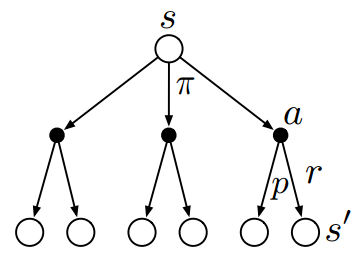
\includegraphics[width=0.3\textwidth]{figs/ch_3_5_1_dackup_diagram_for_vpi.png} 
    \caption{Backup diagram for $v_{\pi}$}
    \label{fig:dackup_diagram_for_vpi}
\end{figure}

\section{Optimal Policies and Optimal Value Functions}
\begin{enumerate}
    \item \textbf{optimal policy:} A policy $\pi$ is defined to be better than or equal to a policy $\pi '$ if its expected return is greater than or equal to that of $\pi '$ for all states. In other words, $\pi \geq \pi '$ if and only if $v_{\pi}(s) \geq v_{\pi '}$ for all $s \in \mathcal{S}$. There is always at least one policy that is better than or equal to all other policies. This is an optimal policy $\pi_{*}$.

    \item \textbf{optimal state-value function:} 
        \begin{equation}
            v_{*}(s) \dot{=} \max_{\pi} v_{\pi}(s) \quad \forall s \in \mathcal{S}
        \end{equation}

    \item \textbf{optimal action-value function:}
        \begin{equation}
            q_{*}(s,a) \dot{=} \max_{\pi} q_{\pi}(s, a) \quad \forall s \in \mathcal{S} \quad and \quad \forall a \in \mathcal{A}(s)        
        \end{equation}
    For the state-action pair $(s, a)$, this function gives the expected return for taking action $a$ in state $s$ and thereafter following an optimal policy.
        \begin{equation}
            q_{*}(s,a) = \mathbb{E}[R_{t+1} + \gamma v_{*}(S_{t+1})|S_t=s, A_t=a]
        \end{equation}

    \item \textbf{Bellman optimality equation for $v_*$:} Intuitively, the Bellman optimality equation expresses the fact that the value of a state under an optimal policy must equal the expected return for the best action from that state. As show in Figure-\ref{fig:backup_diagrams_v_and_q}
    \begin{equation}
    \begin{split}
        v_*(s) = & \max_{a \in \mathcal{A}(s)} q_{\pi_*}(s,a) \\
            = & \max_a \mathbb{E}_{\pi_*}[G_t|S_t=s, A_t=a] \\
            = & \max_a \mathbb{E}_{\pi_*}[R_{t+1} + \gamma G_{t+1}|S_t=s,A_t=a] \\
            = & \max_a \mathbb{E}[R_{t+1} + \gamma v_*(S_{t+1})|S_t=s, A_t=a] \\
            = & \max_a \sum_{s', r} p(s',r|s,a)[r + \gamma v_*(s')]
    \end{split}
    \end{equation}

    \item \textbf{Bellman optimality equation for $q_*$:} As show in Figure-\ref{fig:backup_diagrams_v_and_q}
    \begin{equation}
    \label{eq:bellman_optimality_equation}
    \begin{split}
        q_*(s,a) = & \mathbb{E}[R_{t+1} + \gamma v_*(S_{t+1})|S_t=s, A_t=a] \\
            = & \mathbb{E}[R_{t+1} + \gamma \max_{a'}q_*(S_{t+1}, a')| S_t=s, A_t=a] \\
            = & \sum_{s',r} p(s',r|s, a)[r+ \gamma \max_{a'}q_*(s', a')]
    \end{split}
    \end{equation}
\end{enumerate}
\begin{figure}[htbp]
    \centering
    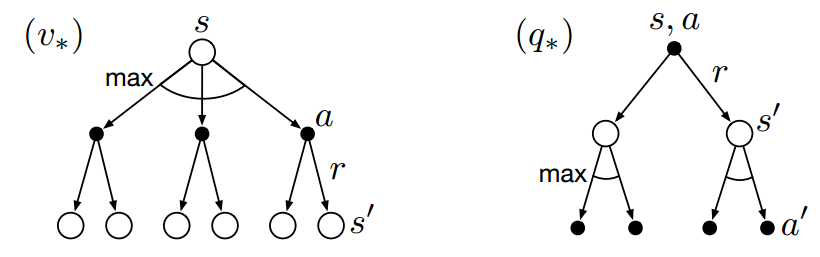
\includegraphics[width=0.6\textwidth]{figs/ch_3_6_1_backup_diagrams_v_and_q.png} 
    \caption{Backup diagram for $v_{*}$ and $q_{*}$}
    \label{fig:backup_diagrams_v_and_q}
\end{figure}

%# -*- coding: utf-8-unix -*-
% !TEX program = xelatex
% !TEX root = ../main.tex
% !TEX encoding = UTF-8 Unicode

\chapter{Dynamic Programming}
\label{chap:ch_4_Dynamic_Programming}
The term dynamic programming (DP) refers to a collection of algorithms that can be used to compute optimal policies given a perfect model of the environment as a Markov decision process (MDP). DP algorithms are obtained by turning Bellman equations such as these into assignments, that is, into update rules for improving approximations of the desired value functions.

\section{Policy Evaluation (Prediction)}
\begin{enumerate}
	\item \textbf{policy evalution(prediction problem):} compute the state-value function $v_{\pi}$for an arbitrary policy $\pi$.
	\item \textbf{iterative policy evaluation:} The existence and uniqueness of $v_{\pi}$ are guaranteed as long as either $\gamma < 1$ or eventual termination is guaranteed from all states under the policy $\pi$.
	\begin{equation}
		v_{\pi}(s) \dot{=} \sum_{a}\pi(a|s)\sum_{s',r}p(s', r|s,a)[r + \gamma v_{\pi}(s')]
	\end{equation}

	\textbf{Update rule:}
	\begin{equation}
	\label{eq:policy_evaluation}
		v_{k+1}(s) \dot{=} \sum_{a}\pi(a|s)\sum_{s',r}p(s', r|s,a)[r + \gamma v_{k}(s')]
	\end{equation}
	Indeed, the sequence $\{v_k\}$ can be shown in general to converge to $v_{\pi}$ as $k \rightarrow \infty$ under the same conditions that guarantee the existence of $v_{\pi}$.

	\item \textbf{expected update:}All the updates done in DP algorithms are called expected updates because they are based on an expectation over all possible next states rather than on a sample next state.

	\item \textbf{In-place iterative policy evaluation:} With two arrays for $v_k(s)$ and $v_{k+1}(s)$ respectively, the new values can be computed one by one from the old values without the old values being changed. Of course it is easier to use one array and update the values “in place,” that is, with each new value immediately overwriting the old one. show in Algorithm-\ref{alg:iterative_policy_evaluation}.
\end{enumerate}

\begin{algorithm}[H]
\label{alg:iterative_policy_evaluation}
\caption{Iterative Policy Evaluation(In-place)}
\begin{algorithmic}[1]
\Require the policy to be evaluated, a small threshold $\theta > 0$ determining accuracy of estimation, Initialize $V(s)$, for all $s \in \mathcal{S}^+$, arbitrarily except that $V(terminal)$=0.
\Statex
\Repeat
	\State \begin{math}\Delta \leftarrow 0\end{math}
	\For{\begin{math} s \in \mathcal{S}\end{math}}
		\State \begin{math}v \leftarrow V(s)\end{math}
		\State \begin{math}V(s) \leftarrow \sum_a \pi(a|s)\sum_{s',r}p(s', r|s, a)[r+\gamma V(s')]\end{math}
		\State \begin{math}\Delta \leftarrow \max(\Delta , |v-V(s)|)\end{math}
	\EndFor
\Until{\begin{math} \Delta < \theta \end{math}}
\end{algorithmic}
\end{algorithm}

\section{Policy Improvement}
\begin{enumerate}
	\item \textbf{policy improvement theorem:} Let $\pi$ and $\pi'$ be any pair of deterministic policies such that, $\forall s \in \mathcal{S}$,
	\begin{equation}
		q_{\pi}(s, \pi'(s)) \geq v_{\pi}(s)
	\end{equation}
	Then the policy $\pi'$ must be as good as, or better than, $\pi$. That is, it must obtain greater or equal expected return from all states $s \in \mathcal{S}$.
	\begin{equation}
		v_{\pi'}(s) \geq v_{\pi}(s)
	\end{equation}

	\item \textbf{policy improvement:} The process of making a new policy that improves on an original policy, by making it greedy with respect to the value function of the original policy. So far we have seen how, given a policy and its value function, we can easily evaluate a change in the policy at a single state to a particular action. It is a natural extension to consider changes at all states and to all possible actions, selecting at each state the action that appears best according to $q_{\pi}(s,a)$. In other words, to consider the new greedy policy, $\pi'$, given by
	\begin{equation}
	\label{eq:policy_improvement}
	\begin{split}
		\pi'(s) \dot{=} & arg \max_{a}q_{\pi}(s,a)\\
			= & arg \max_{a} \mathbb{E}[R_{t+1}+\gamma v_{\pi}(S_{t+1})|S_t=s, A_t=a]\\
			= & arg \max_{a} \sum_{s', r}p(s',r|s,a)[r+\gamma v_{\pi}(s')]
	\end{split}
	\end{equation}

	\item \textbf{optimality:} Suppose the new greedy policy, $\pi'$, is as good as, but not better than, the old policy $\pi$. Then $v_{\pi}=v_{\pi'}$, and from \ref{eq:policy_improvement} it follows that for all $s \in \mathcal{S}$:
	\begin{equation}
	\begin{split}
		v_{\pi'}(s) = & \max_{a} \mathbb{E}[R_{t+1}+ \gamma v_{\pi'}(S_{t+1})|S_t=s, A_t=a]\\
			= & \max_{a} \sum_{s', r}p(s',r|s, a)[r+\gamma v_{\pi'}(s')]
	\end{split}
	\end{equation}
	this is the same as the Bellman optimality equation \ref{eq:bellman_optimality_equation}, and $v_{\pi'}$ must be $v_{*}$, and both $\pi$ and $\pi'$ must be optimal policies. Policy improvement thus must give us a strictly better policy except when the original policy is already optimal.

	\item \textbf{stochastic case:} the ideas of this deterministic case extend easily to stochastic policies.
\end{enumerate}

\section{Policy Iteration}
\begin{algorithm}[H]
\label{alg:policy_iteration}
\caption{Policy Iteration(using iterative evaluation) for estimating $\pi \approx \pi_*$}
\begin{algorithmic}[1]
\Procedure{Initialization}{}
	\State $V(s) \in \mathbb{R}$ and $\pi(s) \in \mathcal{A}(s)$ arbitrarily $\forall s \in \mathcal{S}$
\EndProcedure
\Statex
\Procedure{Policy Evaluation}{}
\label{proc:policy_evaluation}
\Repeat
	\State $\Delta \leftarrow 0$
	\For{\begin{math}s \in \mathcal{S}\end{math}(}
			\State $v \leftarrow V(s))$
		\State $V(s) \leftarrow \sum_{s',r}p(s',r|s, \pi(s))[r+\gamma V(s')]$
		\State $\Delta \leftarrow \max(\Delta, |v-V(s)|)$
	\EndFor
\Until{\begin{math} \Delta < \theta \end{math}}
\EndProcedure

\Statex
\Procedure{Policy Improvement}{}
\State $policy\_stable \leftarrow true$
\For{\begin{math}s \in \mathcal{S}\end{math}}
\State $old_action \leftarrow \pi(s)$
\State $\pi(s) \leftarrow arg \max_{a} \sum_{s',r}p(s',r|s,a)[r+\gamma V(s')]$
\If{\begin{math}old\_action \neq \pi(s)\end{math}}
	\State $policy\_stable \leftarrow false$
\EndIf
\EndFor
\If{\begin{math} policy\_stable \end{math}}
	\State stop and return $V \approx v_*$ and $\pi \approx \pi_*$
\Else
	\State go to \textbf{procedure} \textsc{Policy Evaluation}
\EndIf
\EndProcedure
\end{algorithmic}
\end{algorithm}

\section{Value Iteration}
In fact, the policy evaluation step of policy iteration can be truncated in several ways without losing the convergence guarantees of policy iteration. One important special case is when policy evaluation is stopped after just one sweep (one update of each state).This algorithm is called value iteration, show in Algorithm-\ref{alg:iterative_value_iteration}. It can be written as a particularly simple update operation that combines the policy improvement and truncated policy evaluation steps:
\begin{equation}
\begin{split}
	v_{k+1}(s) \dot{=} & \max_a \mathbb{E}[R_{t+1}+\gamma v_k(S_{t+1})|S_t=s,A_t=a] \\
		= & \max_{a} \sum_{s',r}p(s',r|s,a)[r+\gamma v_k(s')]
\end{split}
\end{equation}
for all $s \in \mathcal{S}$ . For arbitrary $v_0$ , the sequence ${v_k}$ can be shown to converge to $v_*$ under
the same conditions that guarantee the existence of $V_*$.

Another way of understanding value iteration is by reference to the Bellman optimality
equation \ref{eq:bellman_optimality_equation}, Also note how the value iteration update is
identical to the policy evaluation update \ref{eq:policy_evaluation} except that it requires the maximum to be
taken over all actions.

\begin{algorithm}[H]
\label{alg:iterative_value_iteration}
\caption{Value Iteration, for estimating $\pi \approx \pi_*$}
\begin{algorithmic}[1]
\Require the policy to be evaluated, a small threshold $\theta > 0$ determining accuracy of estimation, Initialize $V(s)$, for all $s \in \mathcal{S}^+$, arbitrarily except that $V(terminal)$=0.
\Statex
\Repeat
	\State \begin{math}\Delta \leftarrow 0\end{math}
	\For{\begin{math} s \in \mathcal{S}\end{math}}
		\State \begin{math}v \leftarrow V(s)\end{math}
		\State \begin{math}V(s) \leftarrow \max_a \sum_{s',r}p(s', r|s, a)[r+\gamma V(s')]\end{math}
		\State \begin{math}\Delta \leftarrow \max(\Delta , |v-V(s)|)\end{math}
	\EndFor
\Until{\begin{math} \Delta < \theta \end{math}}
\Statex
\State Output a deterministic policy, $\pi \approx \pi_*$, such that
$$\pi(s)=arg \max_a \sum_{s',r}p(s',r|s, a)[r+\gamma V(s')]$$
\end{algorithmic}
\end{algorithm}

\section{Asynchronous Dynamic Programming}
A major drawback to the DP methods that we have discussed so far is that they involve
operations over the entire state set of the MDP, that is, they require sweeps of the state
set. \textbf{Asynchronous DP algorithms} are in-place iterative DP algorithms that are not organized
in terms of systematic sweeps of the state set. If $0 \leq \gamma < 1$, asymptotic convergence to $v_*$ is guaranteed given only that all states occur in the sequence $\{s_k\}$ an infinite number of  times.

\section{Generalized Policy Iteration}
Letting policy-evaluation and policy improvement processes interact, independent of the granularity
and other details of the two processes. That is, all have identifiable policies and value functions, with the policy always being improved with respect to the value function and the value
function always being driven toward the value function for the policy. If both the evaluation process and the improvement process stabilize, that is, no longer produce changes, then the value function and policy must be optimal.

\section{Efficiency of Dynamic Programming}
DP methods take to find an optimal policy is polynomial in the number of states and actions.DP is sometimes thought to be of limited applicability because of the \textbf{curse of dimensionality}, the fact that the number of states often grows exponentially with the number of state variables. In fact, DP is comparatively better
suited to handling large state spaces than competing methods such as direct search and linear programming.
%# -*- coding: utf-8-unix -*-
% !TEX program = xelatex
% !TEX root = ../main.tex
% !TEX encoding = UTF-8 Unicode

\chapter{Monte Carlo Methods}
\label{chap:ch_5_Monte_Carlo_Methods}
\section{Monte Carlo Prediction}
\begin{enumerate}
	\item \textbf{Monte Carlo methods:} Estimate value function(expected return) from experience, then, is simply to average the returns observed after visits to that state. As more returns are observed, the average should converge to the expected value.

	\item \textbf{First-vist MC method vs every-visit MC method:}  The first-visit MC method, as show in Algorithm-\ref{alg:first-visit_mc_prediction}, estimates $v_{\pi}(s)$ as the average of the returns following \textbf{first visits} to $s$ , whereas the every-visit MC method averages the returns following \textbf{all visits} to $s$. Both first-visit MC and every-visit MC converge to $v_{\pi}(s)$ as the number of visits (or first visits) to $s$ goes to infinity.

	\item \textbf{Property of MC methods:} 
	\begin{enumerate}
	\item The ability of Monte Carlo methods to work with sample episodes alone can be a significant advantage when one has no knowledge or even complete knowledge of the environment’s dynamics;

	\item Monte Carlo methods \textbf{do not bootstrap}, the estimates for each state are independent. The estimate for one state does not build upon the estimate of any other state, as is the case in DP;

	\item The computational expense of estimating the value of a single state is independent of the number of states. 
	\end{enumerate}
\end{enumerate}

\begin{algorithm}[H]
\label{alg:first-visit_mc_prediction}
\caption{First-visit MC prediction, for estimating $V \approx v_{\pi}$}
\begin{algorithmic}[1]
\Require the policy $\pi$ to be evaluated, Initialize $V(s)$, arbitarily, for all $s \in \mathcal{S}$, $Returns(s) \leftarrow $ an empty list, for all $s \in \mathcal{S}$
\Statex
\Loop \Comment{for each episode}
	\State Generate an episode following $\pi$:$S_0, A_0, R_1, S_1, A_1, R_2, \dots, S_{T-1}, A_{T-1}, A_{T-1}, R_T$
	\State $G \leftarrow 0$
	\For{each step of episode, \begin{math}t=T-1, T-2, \dots ,0\end{math}}
		\State $G \leftarrow \gamma G + R_{t+1}$
		\If{\begin{math}S_t\end{math} not in \begin{math}S_0, S_1, \dots, S_{t-1}\end{math}} \Comment{appear in episode for teh first time}
			\State Append $G$ to $Returns(S_t)$
			\State $V(S_t) \leftarrow average(Returns(S_t))$
		\EndIf
	\EndFor
\EndLoop
\end{algorithmic}
\end{algorithm}

\section{Monte Carlo Estimation of Action Values}
\begin{enumerate}
	\item \textbf{Necessity of estimation of action values:} Without a model, state values alone are not sufficient. One must explicitly estimate the value of each action in order for the values to be useful in suggesting a policy.

	\item \textbf{First-visit vs ervery visit MC method:} The every-visit MC method estimates the value of a state–action pair as the average of the returns that have followed all the visits to it. The first-visit MC method averages the returns following the first time in each episode that the state was visited and the action was selected.

	\item \textbf{Maintainig exploration:}  If $\pi$is a \textbf{deterministic policy}, then in following $\pi$ one will observe returns only for one of the actions from each state. However, the purpose of learning action values is to help in choosing among the actions available in each state. To compare alternatives we need to estimate the value of all the actions from each state, not just the one we currently favor. For policy evaluation to work for action values, we must assure \textbf{continual exploration}.

	\item \textbf{Exploring starts:} One way to do this is by specifying that the episodes start in a state–action pair, and that every pair has a nonzero probability of being selected as the start. This guarantees that all state–action pairs will be visited an infinite number of times in the limit of an infinite number of episodes.
\end{enumerate}

\section{Monte Carlo Control(Approximate Optimal Policies)}
\begin{enumerate}
	\item \textbf{Monte Carlo policy iteration:}In this method, we perform alternating complete steps of policy evaluation and policy improvement, beginning with an arbitrary policy $\pi_0$ and ending with the optimal policy and optimal action-value function:
	$$\pi_0 \xrightarrow{E} q_{\pi_0} \xrightarrow{I}
	\pi_1 \xrightarrow{E} q_{\pi_1} \xrightarrow{I} \pi_2 \xrightarrow{E} \dots \xrightarrow{I} \pi_* \xrightarrow{E} q_{\pi_*}$$
	Policy improvement is done by making the policy greedy with respect to the current (action) value function. 
	\begin{equation}
		\pi(s) \dot{=} arg \max_{a} q(s,a)
	\end{equation}
	 The policy improvement theorem then applies to $\pi_k$ and $\pi_{k+1}$ because, for all $s \in \mathcal{S}$,
	 \begin{equation}
	 \begin{split}
	 	q_{\pi_k}(s, \pi_{k+1}(s)) = & q_{\pi_k}(s, arg \max_a q_{\pi_k}(s,a) \\
	 		= & max_a q_{\pi_k}(s,a) \\
	 		\geq & q_{\pi_k}(s, \pi_k(s)) \\
	 		\geq & v_{\pi_k}(s)
	 \end{split}
	 \end{equation}
	 the theorem assures us that each $\pi_{k+1}$ is uniformly better than $\pi_k$ , or just as good as $\pi_k$.

	\item \textbf{Monte Carlo ES:}(Monte Carlo with Exploring Starts)
	
	\begin{algorithm}[H]
	\label{alg:monte_carlo_es}
	\caption{Monte Carlo ES}
	\begin{algorithmic}[1]
	\Require \\Initialize $\pi(s) \in \mathcal{A}(s)$(arbitarily), for all $s \in \mathcal{S}$,\\
	Initialize $Q(s,a) \in \mathbb{R}$(arbitrarily), for all $s \in \mathcal{S}, a \in \mathcal{A}(s)$,\\
	Initialize $Returns(s, a) \leftarrow empty list$, for all $s \in \mathcal{S}, a \in \mathcal{A}(s)$.
	\Statex
	\Repeat
		\State Choose \begin{math} S_0 \in \mathcal{S}, A_0 \in \mathcal{A}(S_0) \end{math} randomly such that all paris have probability \begin{math} > 0 \end{math}

		\State Generate an episode from \begin{math}S_0, A_0\end{math}, following \begin{math} \pi: S_0, A_0, R_1, S_1, A_1, R_2, ..., S_{T-1}, A_{T-1}, R_T\end{math}

		\State \begin{math} G \leftarrow 0 \end{math}

		\For{each step of episode, \begin{math}t=T-1, T-2, ...., 0 \end{math}}
			\State \begin{math}G \leftarrow \gamma G + R_{t+1} \end{math}
			\If{The pair \begin{math}S_t,A_t\end{math} not appears in \begin{math}S_0, A_0, S_1, A_1, ..., S_{t-1}, A_{t-1}:\end{math}}
				\State Append \begin{math} G \end{math} to \begin{math}Returns(S_t, A_t)\end{math}
				\State \begin{math}Q(S_t, A_t) \leftarrow average(Returns(S_t, A_t))\end{math}
				\State \begin{math}\pi(S_t) \leftarrow arg\max_{a}Q(S_t, a) \end{math}
			\EndIf
		\EndFor
	\Until{Converge}
	\end{algorithmic}
	\end{algorithm}
\end{enumerate}

\section{Monte Carlo Control without Exploring Starts}
\begin{enumerate}
	\item \textbf{$\epsilon-soft$ policy:} meaning that $\pi{a|s} > 0$ for all $s \in \mathcal{S}$ and all $a \in \mathcal{A(s)}$, but gradually shifted closer and closer to deterministic optimal policy.

	\item \textbf{On-policy first-visit MC control (for $\epsilon$-soft policies), estimates $\pi \approx \pi_*$}

	\begin{algorithm}[H]
	\label{alg:on_policy_first_visit_MC}
	\caption{On-policy first-visit MC control}
	\begin{algorithmic}[1]
	\Require \\Initialize $\pi \leftarrow$ an arbitrary $\epsilon-soft$ policy\\
	Initialize $Q(s,a) \in \mathbb{R}$ (arbitrarily), for all $s \in \mathcal{S}, a \in \mathcal{A}(s)$\\
	Initialize $Returns(s, a) \leftarrow empty list$, for all $s \in \mathcal{S}, a \in \mathcal{A}(s)$
	\Statex
	\Repeat \Comment{for each episode}
		
		\State Generate an episode following \begin{math} \pi: S_0, A_0, R_1, S_1, A_1, R_2, ..., S_{T-1}, A_{T-1}, R_T\end{math}
		\State \begin{math} G \leftarrow 0 \end{math}
		\For{each step of episode, \begin{math}t=T-1, T-2, ...., 0 \end{math}}
			\State \begin{math}G \leftarrow \gamma G + R_{t+1} \end{math}
			\If{The pair \begin{math}S_t,A_t\end{math} not appears in \begin{math}S_0, A_0, S_1, A_1, ..., S_{t-1}, A_{t-1}:\end{math}}
				\State Append \begin{math} G \end{math} to \begin{math}Returns(S_t, A_t)\end{math}
				\State \begin{math}Q(S_t, A_t) \leftarrow average(Returns(S_t, A_t))\end{math}
				\State \begin{math}A^* \leftarrow arg\max_{a}Q(S_t, a) \end{math}
			\EndIf
				\For{each \begin{math} a \in \mathcal{A}(S_t) \end{math}}
					\If{\begin{math}a = A^*\end{math}} 
						\State \begin{math} \pi(a|S_t) \leftarrow 1-\epsilon+\epsilon/|\mathcal{A}(S_t)| \end{math}
					\Else
						\State \begin{math} \pi(a|S_t) \leftarrow \epsilon/|\mathcal{A}(S_t)| \end{math}
					\EndIf
				\EndFor
		\EndFor
	\Until{Converge}
	\end{algorithmic}
	\end{algorithm}
\end{enumerate}

\section{Off-policy Prediction via Importance Sampling}
\begin{enumerate}
	\item \textbf{off-policy learning:} Use two policies, one is the policy to be learned about and that becomes the optimal policy, called \textbf{target policy}, and one that is more exploratory and is used to generate behavior, called \textbf{behavior policy}.

	\item \textbf{assumption of coverage:} Consider target policy $\pi$ and behavior policy $b$, and both policies are fixed and given. In order to use episodes from $b$ to estimate values for $\pi$, we require that every action taken under $\pi$ is also taken under $b$. That is, we require that $\pi(a|s) > 0$ implies $b(a|s)>0$. It follows from cob=verage that $b$ must be stochastic in states where it is not identical to $\pi$.

	\item \textbf{importance sampling:} a general technique for estimating expected values under one distribution given samples from another. We apply importance sampling to off-policy learning by weighting returns according to the relative probability of their trajectories occuring under target and behavior policies, called the \textbf{importance-sampling ratio}.

	\item \textbf{importance ratio:} given a starting state $S_t$, the probability of subsequent state-action trajectories, $A_t, S_{t+1}, A_{t+1},...,S_T$, occuring under any policy $\pi$ is 
	\begin{equation}
	\begin{split}
	Pr\{A_t, S_{t+1}, A_{t+1},...,S_T|S_t, A_{t:T-1}\sim \pi\} =& \pi(A_t|S_t)p(S_{t+1}|S_t, A_t)\pi(A_{t+1}|S_{t+1})...p(S_T|S_{T-1}, A_{T-1}) \\
	= &\prod_{k=t}^{T-1}\pi(A_k|S_k)p(S_{k+1}|S_k, A_k)
	\end{split}
	\end{equation}
	the relative probability of the trajectory under the target and behavior policies (the importace sampling ratio) is 
	\begin{equation}
	\rho_{t:T-1} \dot{=} \frac{\prod_{k=t}^{T-1}\pi(A_k|S_k)p(S_{k+1}|S_k,A_k)}{\prod_{k=t}^{T-1}b(A_k|S_k)p(S_{k+1}|S_k,A_k)}
	\end{equation}

	\item \textbf{estimating the expected returns (values) under the target policy:} Get returns $G_t$ due to the behavior policy. $v_b(s) = \mathbb{E}[G_t|S_t=s]$, the ratio $\rho_{t:T-1}$ transforms the $v_b(s)$ to $v_{\pi}(s)$.
	\begin{equation}
	\mathbb{E}[\rho_{t:T-1}G_t|S_t=s]=v_{\pi}(s)
	\end{equation} 

	\item \textbf{ordinary importance sampling:} To estimate $v_{\pi}(s)$, we simply scale the returns by the ratios and avrage the results
	\begin{equation}
	V(s) \dot{=} \frac{\sum_{t \in \mathcal{J}(s)}\rho_{t:T(t)-1}G_t}{|\mathcal{J}(s)|}
	\end{equation}

	\item \textbf{weighted importance sampling:}
	\begin{equation}
	V(s) \dot{=} \frac{\sum_{t \in \mathcal{J}(s)}\rho_{t:T(t)-1}G_t}{\sum_{t \in \mathcal{J}(s)\rho_{t:T(t)-1}}}
	\end{equation}

	\item \textbf{difference between the two importance sampling:} for the first-visit methods, ordinary importance sampling is unbiased whereas weighted importance sampling is baised (though the bias convergesasymptotically to zero).On the other hand, the variance of ordinary importance sampling is in general unbounded because the variance of the ratios can be unbounded, whereas in the weighted estimator the largest weight on any single return is one. In fact, assuming bounded returns, the variance of the weighted importance-sampling estimator converges to zero even if the variance of the ratios themselves is infinite. The every-visit methods for ordinary and weighed importance sampling are both biased, though, again, the bias falls asymptotically to zero as the number of samples increases.

\end{enumerate}
\part{Approximate Solution Methods}


%----------------------------------------------------------------------------------------
%   BIBLIOGRAPHY
%----------------------------------------------------------------------------------------

\bibliographystyle{unsrt}

\bibliography{bib/reference}

%----------------------------------------------------------------------------------------

\end{document}